\documentclass[a4paper,parskip,headheight=38pt]{scrartcl} % article or scrartcl
\usepackage[utf8]{inputenc}
\usepackage[T1]{fontenc}
\usepackage{amsmath,amssymb,amsfonts}
\usepackage[%
  automark,
  headsepline                %% Separation line below the header
]{scrlayer-scrpage}
\usepackage[english]{babel}
\usepackage{hyphenat}
\usepackage[hidelinks]{hyperref}
\usepackage[top=1.4in, bottom=1.5in, left=1in, right=1in]{geometry}
\usepackage{lastpage}
\usepackage{csquotes}
\usepackage{microtype}
\usepackage{datetime}

\usepackage[normalem]{ulem}
\usepackage{enumerate}
\usepackage{hyperref}

% \usepackage{multicol}
\usepackage{graphicx}
\usepackage{graphics}
% \usepackage{float}
% \usepackage{caption}

\setkomafont{pagehead}{\normalfont\sffamily\footnotesize}
\addtolength{\headheight}{+6pt}
\lohead{Marlene Böhmer, s9meboeh@stud\ldots, 2547718 \\
	Maximilian Köhl, mail@koehlma.de, 2553525 \\
	Ben Wiederhake, s9bewied@stud\ldots, 2541266}
\rohead{\newline \newline ES16, Set 2, Page {\thepage}/{\pageref*{LastPage}}}

\newtimeformat{mytime}{\twodigit{\THEHOUR}\twodigit{\THEMINUTE}\twodigit{\THESECOND}}
\settimeformat{mytime}
\newdateformat{mydate}{\twodigit{\THEYEAR}\twodigit{\THEMONTH}\twodigit{\THEDAY}}
\cfoot{\tiny\texttt{ID \mydate\today\currenttime}}
\chead{} % Needed because now the \subsections get displayed
\pagestyle{scrheadings}

% \renewcommand{\headrulewidth}{0pt}
% \addtolength{\textheight}{+30mm}
% \addtolength{\textwidth}{+50mm}
% \addtolength{\hoffset}{-7mm}

% \newcommand{\Omicron}{\ensuremath{\mathcal{O}}}
% \newcommand{\omicron}{\ensuremath{o}}
% \newcommand{\set}[1]{\{#1\}}
% \newcommand{\abs}[1]{\lvert #1 \rvert}

\DeclareMathOperator{\sinc}{sinc}

\begin{document}

\section*{Problem 1: Sampling}

\subsection*{Part 1}

See file \texttt{p1a\_model.mdl}

\subsection*{Part 2}

By the sampling theorem, any sampling rate strictly greater than 4kHz
(2 times the maximum input frequency) is fine.  Thus, the minimal
reconstructing sampling rate is $2 + \varepsilon$ kHz, where
$\varepsilon$ is the minimal increment.

The limiting factors are: imprecise and inaccurate measurements; clock
drift; clock drift (and thus slightly off frequencies) in the input
signal; only a finite set of samples is available (possibly only the
\emph{past} samples).

\subsection*{Part 3}

Using Matlab, one can easily compute the samples:
 %
\begin{verbatim}
>> t = 0:.5:3;
>> sin(pi * t - 1/4)
   -0.2474    0.9689    0.2474   -0.9689   -0.2474    0.9689    0.2474
>> sin(2 * pi * t - 1/4)
   -0.2474    0.2474   -0.2474    0.2474   -0.2474    0.2474   -0.2474
\end{verbatim}

Then the reconstructed signals $\hat{f}$ and $\hat{g}$ are:
 %
\begin{align*}
    \hat{f}(t) &= \sin(\frac{-1}{4}) \cdot \left(\sinc(t -0) - \sinc(t - 1) + \sinc(t-2) - \sinc(t - 3) \right) \\
    &\quad + \sin(\pi \cdot \frac{1}{2} - \frac{1}{4}) \cdot \left( \sinc(t - 0.5) - \sinc(t - 1.5) + \sinc(t - 2.5) \right) \\
    \hat{g}(t) &= \sin(\frac{-1}{4}) \cdot \left(\sinc(t -0) - \sinc(t - 0.5) + \sinc(t - 1) - \sinc(t - 1.5) \right. \\
    &\qquad\qquad\qquad + \left. \sinc(t-2) - \sinc(t-2.5) + \sinc(t - 3) \right)
\end{align*}

Per definition (see slides), we know that $\sinc(x) =
\frac{\sin\left(\frac{\pi}{p_s}x\right)}{\frac{\pi}{p_s}x}$ and from
the exercise that $p_s = 0.5$.  Thus we get these plots:
 \\
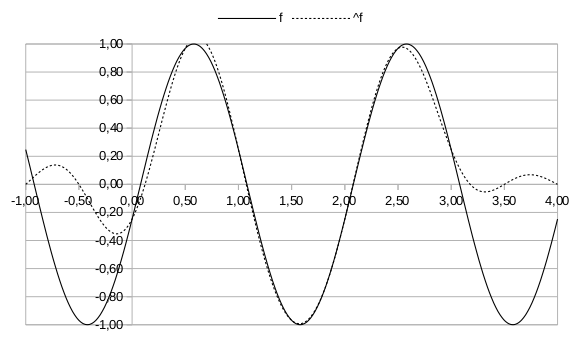
\includegraphics[width=\textwidth]{p1c_f}
 \\
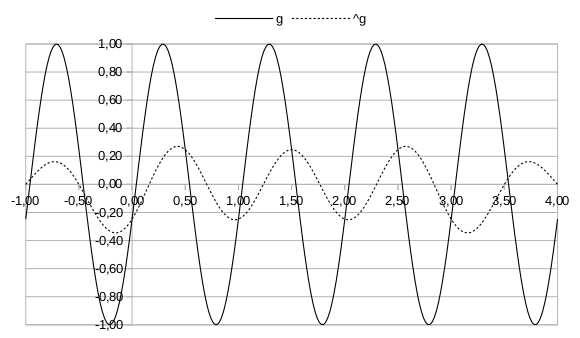
\includegraphics[width=\textwidth]{p1c_g}

For $f$, the approximation is reasonably close in the sampled region,
as there are enough samples.  Outside the sampled region, $\hat{f}$
deviates, mostly by falling towards zero: this is to be expected due to
the missing samples.
 \\ % Squeeze on the same page
$g$ and $\hat{g}$ are pretty far apart, with only the frequency being
correct.  Amplitude and phase couldn't be reconstructed properly as the
sampling frequency is not \emph{strictly} greater than twice the input
frequency.


\section*{Problem 2: Linear System}

\subsection*{Part 1}

First of all, compute $A$ as a matrix:

\begin{align*}
    A &= \left( \begin{array}{cc} 0 & 1 \\ -2 & -3 \end{array} \right) \\
    \det(A - \lambda I) &= (-\lambda)(-3-\lambda) + 2 \\
    &= \lambda^2 + 3\lambda + 2 \\
    \implies \lambda_{1,2} &= \{-1, -2\} \\
    \implies J &= \left( \begin{array}{cc} -1 & 0 \\ 0 & -2 \end{array} \right) \\
    Av_1 &= \lambda_1 v \\
    \iff \binom{v_{1,2}}{-2v_{1,1}-3v_{1,2}} &= \binom{-v_{1,1}}{-v_{1,2}} \\
    \iff v_{1,2} &= -v_{1,1} & \text{e.g. } v_1 = \binom{1}{-1} \\
    Av_1 &= \lambda_2 v \\
    \iff \binom{v_{2,2}}{-2v_{2,1}-3v_{2,2}} &= \binom{-2v_{2,1}}{-2v_{2,2}} \\
    \iff v_{2,2} &= -2 v_{2,1} & \text{e.g. } v_2 = \binom{1}{-2} \\
    \implies P &= \left( \begin{array}{cc} 1 & 1 \\ -1 & -2 \end{array} \right) \\
    \implies P^{-1} &\overset{\text{\scriptsize{matlab}}}{=} \left( \begin{array}{cc} 2 & 1 \\ -1 & -1 \end{array} \right) \\
    \implies \bar{S}(t) &= P D(e^{-t}, e^{-2t}) P^{-1} s_0
\end{align*}

\subsection*{Part 2}

From the result $\lambda_{1,2} = \{-1, -2\}$ one can directly see that
the system is asymptotically stable, as all eigenvalues are strictly
negative.


 \pagebreak{}
\section*{Problem 3: Power Management}

FIXME


\section*{Problem 4: Pendulum}

FIXME


\end{document}
